% !TeX root = ../main.tex
\chapter{SLAM设计和实现}
一个SLAM系统的设计和实现是十分考究代码功底的。按流程一步步走确实能够写出一套能用的东西出来,但是再往上填东西就显得十分吃力。不仅如此,每张图片进入视觉历程计中都会产生上千个特征点每个特征点中一部分有对应的三维地图点,这些地图点又关联着每一个能够观测到它的图片,在BA的过程中还需要全局每一帧每一个地图点捆绑调整。点,图片,位姿,相机之间关系错综复杂,若是不能准确的理清之间的关系,很难编写出一套可用的SLAM框架。\par
除了逻辑上的困难,再一方面的困难就是编程语言上的困难。C++作为一门静态语言,在编写程序的时候要做好内存管理,线程安全等工作。将一个局部变量的地址传出去,释放或者访问已经被释放的内存空间等等这些问题对于初学者来说一不留神都可能遇到。而这些问题都是可以通过一定的编程规范来解决的,比如通过shared\_ptr或者unique\_ptr来保证内存的安全释放,绝不把回传局部变量的地址等等。好在C++11以及后续标准的不断提出,给人们编写大规模程序提供了更多安全上的保障。同时11标准还给C++添加了许多语法糖比如lambda表达式,auto,模板自动推导类型等等都让程序编写起来更加优雅易读。\par
\begin{figure}[H]
	\centering
	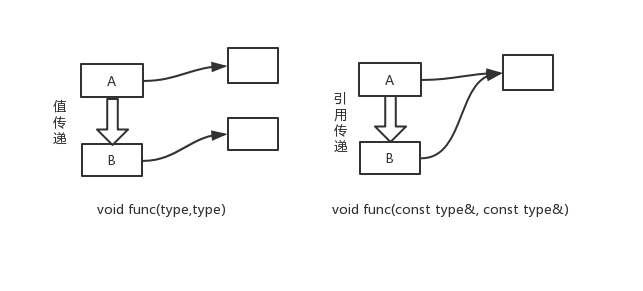
\includegraphics[height=7cm]{byvalueref}
	\caption{值传递和引用传递}
\end{figure}
再一方面就是效率上的问题,C++中函数的传入需要形参,这会使传入的量执行一次拷贝构造函数,同样的,在函数返回的时候要将返回值先执行一次拷贝构造函数,再把旧返回值析构掉。对于系统内置变量,这样的操作影响不大。但是对于用户自定义的类,特别是包含大量数据(比如图片)的成员变量来说,执行拷贝的代价是不可忍受的。因此我们可以采用const \&的方式来进行引用传递。或者可以让类不保存大型数据的实体,只保存地址以节省空间。在执行拷贝构造函数的时候只付出了拷贝地址的代价而不必拷贝实体。这些都能使程序的运行更加流畅。\par
SLAM是个增量式系统,图片会源源不断的读进程序中,如何保证程序不因为读入太多图片而导致内存爆炸,还需要及时从内存中释放掉一部分图片,考虑在相机静止不动的时候,由于一直有图片输入,系统就会不断地进行计算。我们肯定不希望整个模型变得越来越大,因此我们提出了关键帧的概念。对于非关键帧来说,它们的加入只是提供地图点然后就可以释放掉地图,而关键帧则需要留给后端做仔细的优化。\par
总之在实现一个SLAM系统的过程中,需要考虑的零零碎碎的东西非常之多,鉴于毕业设计时间仓促,并没有亲手实现出一整套SLAM系统。但是借助于航空学院赵勇博士的DIYSLAM\cite{zhao2019gslam}优秀的模块化设计,我得以实践SLAM中的很多模块。\par
\begin{figure}[H]
	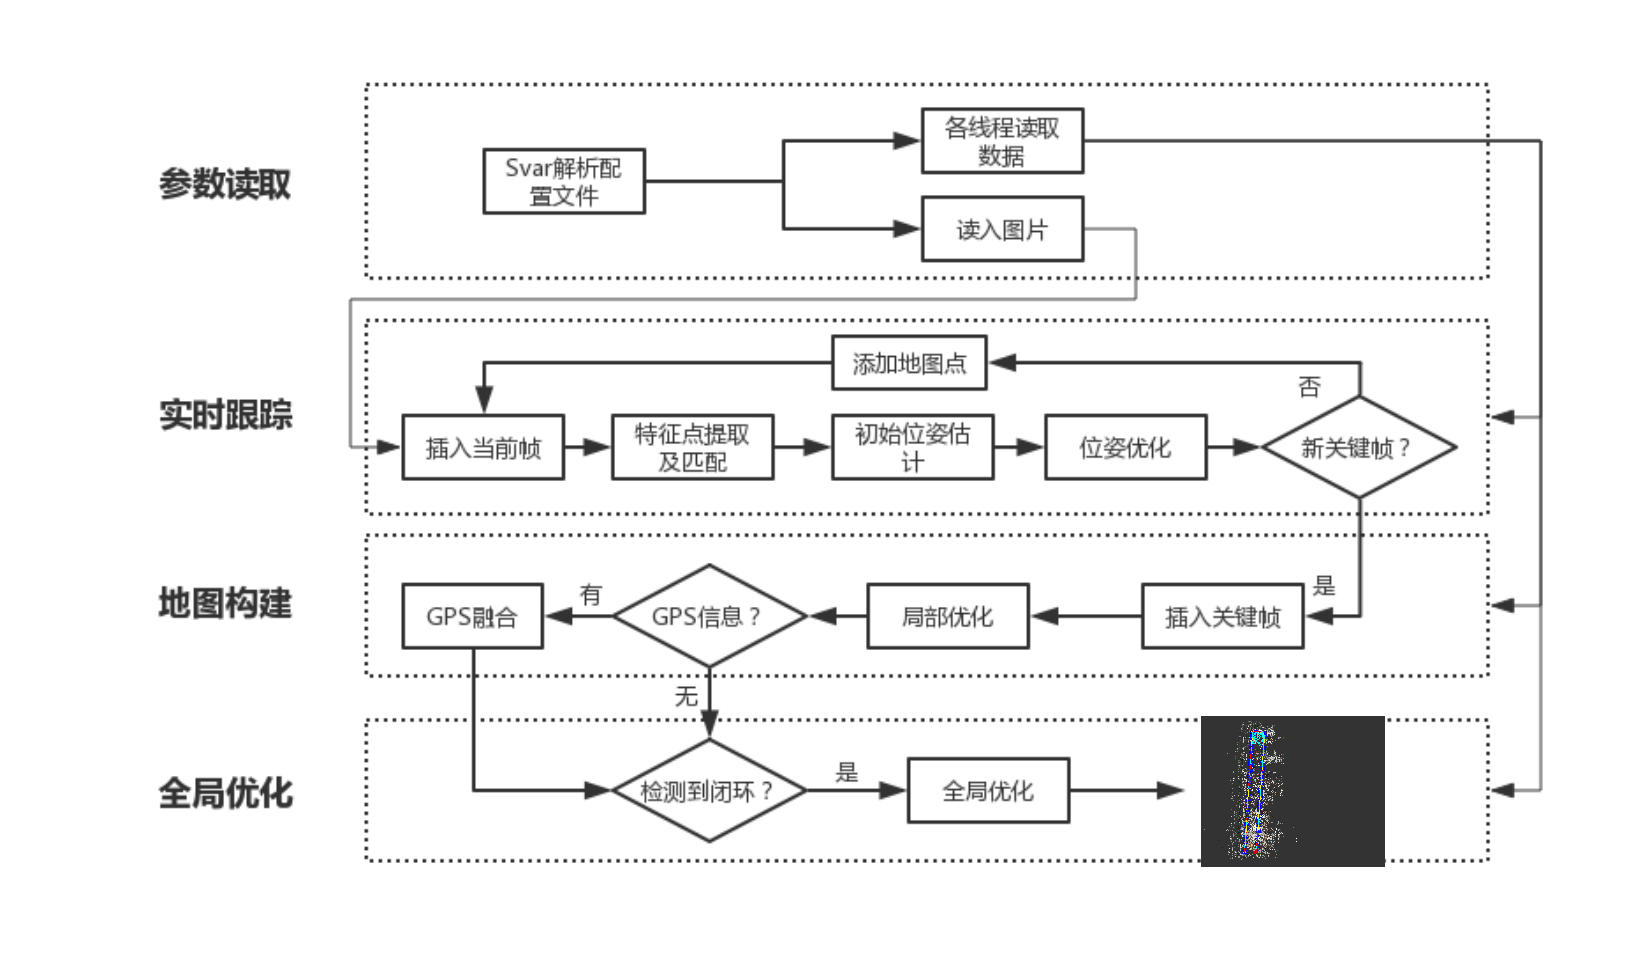
\includegraphics[height=9cm]{liucheng}
	\caption{SLAM设计流程}
\end{figure}
下面就简单介绍一下SLAM的模块以及设计细节
\section{Svar及其应用}
Svar\footnote{https://github.com/zdzhaoyong/Svar}是一个致力于将C++变成高性能动态语言中介,类似于Pybind11,但是能提供更多动态语言的接口。本次设计过程我们将利用Svar进行配置文件解析以及全局参数配置的过程。\par
\begin{table}[]
	\centering
	\caption{Svar参数概览}
	\begin{tabular}{ll}
		\toprule
		\textbf{Key}                    & \textbf{Value}                       \\ \midrule
		FeatureDetector                 & ORB                                  \\ \hline
		Map                             & Hash                                 \\ \hline
		Matcher                         & c\_Flann                             \\ \hline
		Tracker            & opt              \\ \hline
		Initializer                      & opt\_svd  \\ \hline
		SLAM.nFeature                   & 1000                                 \\ \hline
		SLAM.Vocabulary                 & orb\_10\_5\_tfidf\_l1.gbow           \\ \hline
		Mavic\_Pro\_1280\_720.Paraments & {[}1280 720 1028.8 1028.8 640 360{]}                               \\ \bottomrule
	\end{tabular}
\end{table}
我们在Svar中配置了自己的FeatureDetector,Matcher和Initializer等项,除此之外还设置了相机的内参K,以及词袋模型中预先训练好的词袋等等。
\section{特征点匹配}
我们在前面介绍了很多特征点,现在我们就来看一下各种特征点的提取耗时和描述子的计算耗时情况。
\begin{table}[htbp]
	\centering
	\caption{特征点提取时间比较}
	\begin{tabular}{cccc}
		\toprule
		类型    & 总耗时(ms) & 特征点数  & 单个特征点提取时间(ms) \\ \midrule
		FAST   & 46.16   & 70829 & 0.0006        \\ \hline
		SIFT   & 3599.76 & 23458 & 0.1534        \\ \hline
		SURF   & 2761.82 & 43029 & 0.0641        \\ \hline
		ORB    & 114.77  & 500   & 0.2295        \\ \hline
		HARRIS & 439.42  & 1000  & 0.4394      	\\ \bottomrule
	\end{tabular}
\end{table}\par

\begin{table}[]
	\centering
	\caption{描述子计算时间比较}
	\begin{tabular}{cccc}
		\toprule
		类型   & 总耗时(ms) & 特征点数 & 单个特征点描述子计算时间(ms) \\ \midrule
		SIFT  & 958.15  & 500  & 1.9163           \\ \hline
		SURF  & 227.97  & 500  & 0.4559           \\ \hline
		ORB   & 144.90  & 500  & 0.2898           \\ \hline
		BRIEF & 26.46   & 500  & 0.0529          \\ \bottomrule
	\end{tabular}
\end{table}
从上表来看,对于特征点的提取来说,表现最好的是FAST特征点,而在描述子的计算上BRIEF描述子计算速度最快。但是我们并不选用这个两个方法来计算特征点,选用FAST+BRIEF的方式并不具有旋转不变性和尺度不变性。事实上ORB方法正是为了解决这个问题来创造出来的,ORB在速度上的表现也不错,因此我们选用ORB方法来进行特征点的提取。\par
下一步是选取特征点匹配策略,通过图\ref{filters}的结果来看,采用FLANNMather+RANSAC+Lowe's algorithm+交叉过滤等多重保障来保证匹配的正确性。因为对于SLAM系统来说,正确的匹配非常之重要。
\section{跟踪}
在特征点匹配完毕之后对于单目摄像机我们还要进行初始化操作,具体参照第六章视觉历程计。初始化完毕我们就确定了尺度问题,之后再输入的图片我们就重复上述的匹配流程,根据匹配结果利用PnP-RANSAC算法来求解相邻两帧的运动。但是这样做还是有些耗时,我们考虑用以下策略来快速找到匹配:
\begin{enumerate}
	\item 匀速率运动模型:假设摄像头作直线运动,这样我们就能通过上一帧的位姿和速度来对当前帧的位姿进行估计。然后再将地图中的3D点根据当前摄像头的位姿投影到像素平面,并在投影点的附近进行搜索看是否能找到距离比较近的点。如果能,则认为这两者是一个匹配。然后再根据这些3D-2D匹配利用PnP计算位姿。
	\item 关键帧模型:如果上述的匀速率运动模型失败,那么我们试着与最近的关键帧做匹配,使用词袋模型来加速匹配。首先它计算当前帧的词袋,并将上一帧的位姿作为初始化位姿,然后根据位姿和词袋将找到的特征进行匹配,最后利用匹配的特征优化位姿。
	\item 重定位:假设我们用上述的方法都无法匹配,这个时候就需要重定位。此时,我们将当前帧和地图中的所有关键帧进行匹配,以求找到正确的位姿。它先计算当前帧的词袋向量,然后再词袋中选取一些关键帧,然后再次寻找有充足数量可以用于匹配的特征点的关键帧,最后进行匹配迭代解算位姿。  
\end{enumerate}
\subsection{局部地图跟踪}
通过前面的跟踪过程,已经对当前帧位姿有了一个初始估计,接下来我们就可以通过投影搜索局部地图点云的匹配。根据匹配优化位姿和空间三维点位置。所为局部地图,指的是在当前帧视野范围内的3D点。我们会时时更新这个局部地图。\par
从局部地图里进行投影从而找到匹配的过程是这样的:
\begin{enumerate}
\item 把局部地图投影到当前帧,舍弃超出当前帧范围的地图点。
\item 舍弃点云平均视线方向向量$\overrightarrow{\mathbf{n}}$与当前视线方向向量$\overrightarrow{\mathbf{v}}$角度大于60°的点云。
\item 舍弃点云上深度d在$\left[d_{\min }, d_{\max }\right]$范围之外的点。
\item 将剩下的3D点对应的描述子和当前帧还未匹配的ORB描述子进行匹配,找到更多匹配关系。
如果当前帧是关键帧的话,机器人进行之后会进行局部BA来优化位姿,局部地图的三维点以及具备共视关系的帧的位姿。
\end{enumerate}
\subsection{关键帧的判断}
在局部地图中,为了保证计算和存储资源分配,需要舍弃多余的关键帧,与此同时还需要插入新的关键帧,以保证系统的鲁棒性。我们根据下面的标准判断当前帧是否为关键帧:\par
\begin{enumerate}
\item 距离上次全局重定位已超过20帧。
\item 距离上次插入新关键帧或者停暂停建局部地图已超过20帧。
\item 当前帧匹配上超过50个特征点。
\item 当前帧跟踪到的特征点比参考关键帧少90\%。
\end{enumerate}
\section{局部建图}
在跟踪后,我们插入了新的关键帧,下面就需要做多余地图点和关键帧的剔除,还有Local BA,下面进行简单介绍:\par
\begin{enumerate}
	\item 检查队列中是否有需要处理的关键帧。
	\item 计算关键帧的词袋,将关键帧插入地图。
	\item 剔除质量不好的局部地图点。
	\item 生成一些局部地图点。
	\item 融合当前关键帧和相邻关键帧重复的局部地图点。
	\item 处理完队列中的关键帧,如果地图中的关键帧大于2,则进行局部BA优化。
	\item 剔除多余的关键帧。
\end{enumerate}
完成上述工作后,关键帧就会被记录到数据库列表中,我们就完成了Mapping的工作。\par
经过各项函数用时结果参见附录A。
\begin{figure}
	\centering
	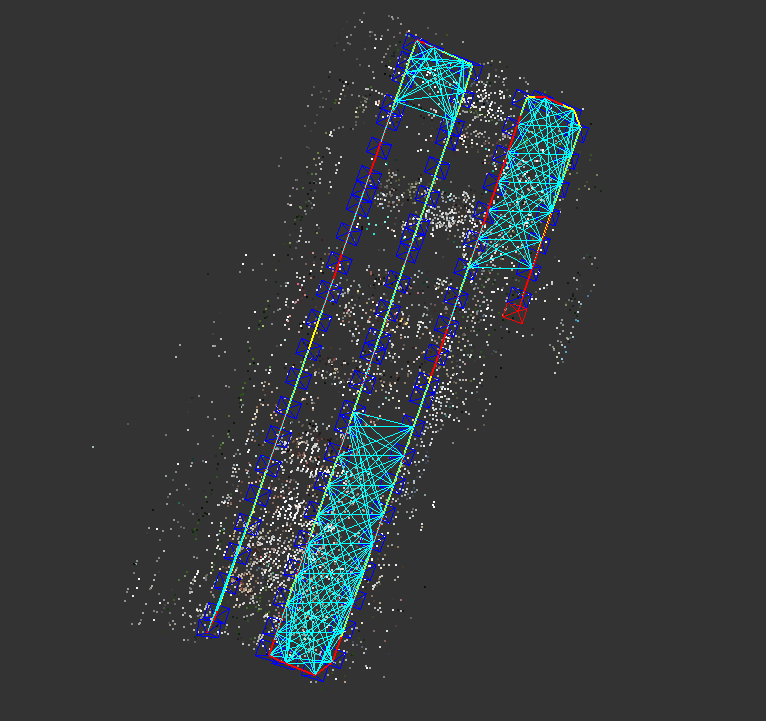
\includegraphics[height=10cm]{runtimecapture}
	\caption{DIYSLAM运行截图}
\end{figure}










